% Created 2019-07-15 Mon 20:26
\documentclass[a4paper,twocolumn]{article}
\usepackage[utf8]{inputenc}
\usepackage[T1]{fontenc}
\usepackage{fixltx2e}
\usepackage{graphicx}
\usepackage{longtable}
\usepackage{float}
\usepackage{wrapfig}
\usepackage{rotating}
\usepackage[normalem]{ulem}
\usepackage{amsmath}
\usepackage{textcomp}
\usepackage{marvosym}
\usepackage{wasysym}
\usepackage{amssymb}
\usepackage{hyperref}
\tolerance=1000
\usepackage[citestyle=authoryear-icomp,bibstyle=authoryear,hyperref=true,backref=true,maxcitenames=3,url=true,backend=biber,natbib=true]{biblatex}
\addbibresource{IterativeKD.bib}
\setcounter{secnumdepth}{2}
\author{Sharan Yalburgi}
\date{\today}
\title{Iterative Knowledge Distillation}
\hypersetup{
  pdfkeywords={},
  pdfsubject={},
  pdfcreator={Emacs 25.2.2 (Org mode 8.2.10)}}
\begin{document}

\maketitle

\section{Abstract}
\label{sec-1}
Deep (Convolutional) Neural Networks have recently shown remarkable success in many real-world visual recognition tasks. These networks are defined with very deep structure (hidden layers and neurons) and numerous model parameters (weights). This makes the existing deep neural network models computationally expensive and memory intensive. Such expensive models find very limited application when it comes to their deployment in devices with lower memory resources or applications with strict latency requirements. Therefore, a straightforward idea is to compress these deep models and accelerate the training process without significantly degrading the original model performance. In this paper, we develop an approach of recursively generating student models (compressed models) from the teacher models (original model and subsequently the compressed models). Each student model is trained with a composite loss function consisting of three different functional terms: KL-divergence between output logits of student and the teacher model, the cross-entropy loss with true labels, and additionally a hint from the teacher model. We also demonstrate the student model building as a search procedure. The recursive building of student (compressed) models stops when there is a significant drop in the performance. We evaluate our model compression approach for compressing Deep Convolutional Neural Networks (CNN) for two well-known benchmark datasets such as MNIST digits dataset and CIFAR-10 dataset. Experimental results demonstrate that our proposed approach can compress original Deep-CNN model with x\% reduction in memory footprint with y\% drop in performance as compared with the original model. These results are comparable/better to/than the state-of-the-art model compression methods.
\section{Introduction}
\label{sec-2}
Problem Statement: What is the problem? Why is it important to solve
it? How do we intend to solve it?

Deep Neural Networks have achieved remarkable results in the recent
past. They have been applied in various fields including medical
diagnosis, finance, drug discovery, speech recognition and space
exploration to name a few.

However, they often have hundreds of millions of parameters. Hence
take several days to train even on high performance GPUs. This not
just slows down the initial training procedure but also is burden
while eventually deploying on real time system where predictions are
often required to almost instantaneous with little resource..

As we entertain larger and larger neural networks to model our data,
it becomes more important to consider its storage and computational
requirements. Especially in the context of real time systems we need
models to perform with less resource both in terms of computation and
storage. Another aspect which is of importance in remote embedded
systems is power consumption.

We will restrict or investigation to storage and computation in this report.

\section{Model Compression}
\label{sec-3}

Model compression is the process of modifying or using a trained model
to create a new model which generally takes lesser computation and/or
storage and/or power but retains comparable performance.

There are several existing techniques for model compression. Some of
them include parameter pruning, low-rank factorization, knowledge
distillation to name a few.

We focus on the idea of model compression by knowledge distillation in
this report.

\subsection{Knowledge Distillation}
\label{sec-3-1}

\textbf{Knowledge Distillation} is the idea of complex model
transferring its learnt knowledge to a less complex model. We aim to
match the original model's performance in the learnt model. Throughout
this report we use the terminology that \textit{parent model} is
teaching the \textit{child model}. We use the term \textit{ancestors}
to refer to any and all models which are used to train a specific
model.

The idea Knowledge Transfer was first proposed in
\cite{bucilua2006model}. A more recent work first applied it to deep
neural networks.\cite{ba2014deep}

\subsection{Iterative Knowledge Distillation}
\label{sec-3-2}
The key idea of iterative knowledge distillation is to gradually reduce the model size by using a parent model(s) to train a child mode(s). Throughout this process the of learning and re-learning we keep the algorithm exposed to the data. We have seen that this at times increases the performance with child model(s).

We propose several variations of Iterative Knowledge Distillation.

\subsubsection*{Parent $\rightarrow$ Child}
\label{sec-3-2-1}
This is simplest version of Iterative Knowledge Distillation where a single parent teaches a single child. This process could be repeated until the drop in the performance is within reasonable amounts.

\subsubsection*{Parent $\rightarrow$ Children}
\label{sec-3-2-2}
In this variation we propose in ensemble learning approach where at each learning phase, we train an ensemble of children using a single parent. The children could be of same architecture with different initialisations or could have different architectures. We could select the best performing child at each step before performing the next iteration of Knowledge Distillation or we could grow a tree of Parent-Child models. 

\subsubsection*{Ancestors $\rightarrow$ Child}
\label{sec-3-2-3}
We propose that several expert Parent models could be used to train a single Child model. The parent could have different architectures catering to different aspects of the data. 

\subsubsection*{Ancestors $\rightarrow$ Children}
\label{sec-3-2-4}
This the a development over the previous approach where several expert Parent models could help train a several Child models. We could select the best performing child at each step before performing the next iteration of Knowledge Distillation or we could grow a tree of Ancestors-Children models.

\section{Empirical Evaluation}
\label{sec-4}

\subsection{Data}
\label{sec-4-1}

We consider two of the most popular datasets in vision. MNIST and CIFAR-10

\subsubsection*{MNIST}
\label{sec-4-1-1}
\textbf{MNIST}\parencite{mnist} is a dataset of handwritten digits. It hence has 10 classes. It has training set of 60,000 digits and test set of 10,000 digits. All digits are greyscale images of dimensions 28x28. The digits have been size-normalized and centered in a fixed-size image. Each class has been equally represented in the train and test set.

\subsubsection*{CIFAR-10}
\label{sec-4-1-2}
\textbf{CIFAR-10}\parencite{cifar} is a dataset of 10 classes. It has training set of 50,000 digits and test set of 10,000 digits. All digits are RGM images of dimensions 32x32. Each class has been equally represented in the train and test set. The classes are completely mutually exclusive. The dataset contains common objects like animals and automobiles.

\subsection{Model Compression for MNIST and CIFAR-10}
\label{sec-4-2}

To demonstrate model compression, we compress models trained on MNIST and CIFAR-10 to the smallest possible size. We consider VGG-16 and VGG-19 models as our initial trained models. We two different compression strategies.

\subsubsection*{Reduce number of Blocks}
\label{sec-4-2-1}
Here we reduce the number of blocks in the VGG-16 and VGG-19 network in a gradual manner.

\subsubsection*{Reduce Block Size}
\label{sec-4-2-2}
We reduce the complexity blocks in the VGG-16 and VGG-19 network in a gradual manner.


\subsection{Loss Function}
\label{sec-4-3}

$LOSS = KLDivergence(ParentModel, ChildModel) + CrossEntropyLoss(Y, \hat{Y})$


\section{Results}
\label{sec-5}

\begin{figure}[htb]
\centering
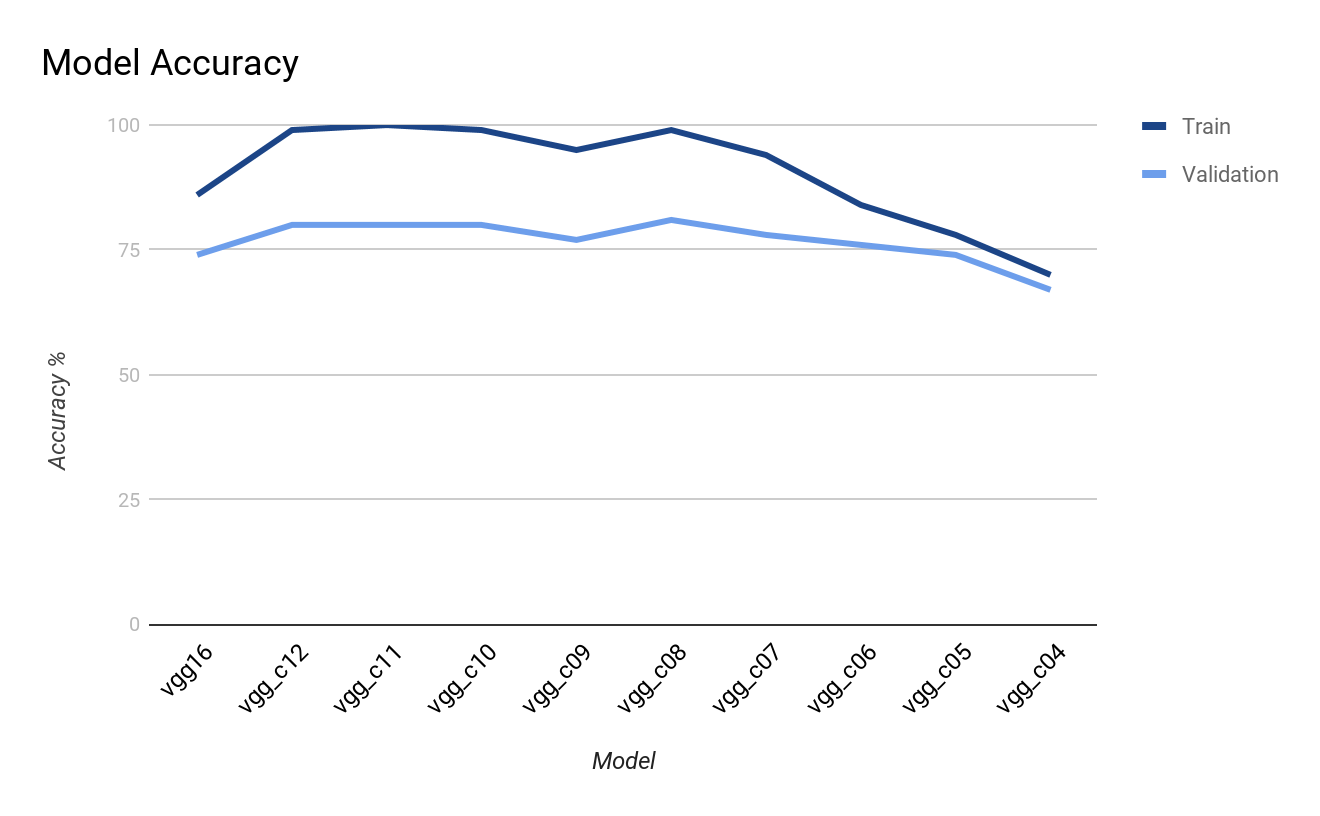
\includegraphics[width=.9\linewidth]{./media/vgg16-cifar10/vgg16_cifar10_Acc.png}
\caption{\label{fig:SED-HR4049}This is the caption for the next figure link (or table)}
\end{figure}

\section{Conclusion}
\label{sec-6}


\printbibliography
% Emacs 25.2.2 (Org mode 8.2.10)
\end{document}
